\chapter{Wahl der Metrik}\label{chap:Wahl_der_Metrik}
\section{Klassische Metriken}
Bei der Berechnung jeder Metrik gehen Informationen verloren, da zwei zeitliche Signale, welche jeweils komplizierte Zusammenhänge zwischen den einzelnen Events haben, auf eine reelle Zahl abgebildet werden. 
Also sollte man genau betrachten, welche Informationen bei dem Berechnen der klassischen Metriken verloren gehen.

Das Ziel der poysomnographischen Untersuchung und Auswertung ist es, die klinischen Kennzahlen der AASM \cite{AASM} aus dem Annotationssignal zu bestimmen, um herauszufinden, wie stark ein Krankheitsverlauf den Schlaf stört. Daher wäre es sinnvoll den Detektor an dem Vergleich dieser Kennzahlen zu bemessen.
Der Vergleich der Kennzahlen liefert allerdings kein vollständiges Bild über die korrekte Arbeitsweise des Detektors. Die Kennzahlen werden bei dem Detektor aus \gls{TP}- und \acrfull{FP} Werten berechnet. Letztere sind allerdings nicht durch eine korrekte Arbeitsweise entstanden, sondern durch einen Fehler des Detektors.


Für die Bewertung des Annotationssignales kann die Berechnung von \gls{TP}, \gls{FP}, \gls{TN} und \gls{FN} Werten segementweise oder eventweise geschehen. 

Selbst bei einer schweren Erkrankung mit einem PLM-Index von 60 pro Stunde \cite{PDS} und maximaler Beinbewegungslänge von zehn Sekunden liegt das Verhältnis von Beinbewegungen zu Ruhephasen bei circa eins zu fünf. Bei einer segmentweisen Berechnung hätte also eine starke Ungleichverteilung in beiden Klassen. Da die Anzahl der TN sehr hoch sein wird, bieten Sensitivität, Spezifität, und Korrektklassifikationsrate keinen informativen Gehalt \cite{Huang}. 
Die Länge der jeweiligen LM ist für medizinische Entscheidungen nicht relevant. Da nur die Anzahl (und Abstände) der Events zählen, ist es sinnvoller die Metriken eventbasiert zu berechnen.
Bei dieser zählweise sind die Klassen wesentlich gleicher verteilt, da gilt: TP + FP + 1 = TN + FN (falls die Ränder negativ sind). 

Die Metriken, die sich anhand des Annotationssignales berechnen lassen, sind eher ungeeignet, um einem Detektor eine Güte zuzuweisen. Bei den Metriken Genauigkeit, Spezifizität und negativem Vorhersagewert fehlt jeweils eine der vier Klassen, weswegen die Werte einzeln betrachtet den Detektor nicht gut repräsentieren. Beispielsweise wäre die Sensitivität perfekt auf dem Wert 1 wenn der Detektor jeden Abtastwert als Beinbewegung klassifiziert. 
Es kann außerdem passieren, dass die klassischen Metriken unendlich große Werte annehmen beziehungsweise neu definiert werden müssten.
Dies kommt zum Beispiel bei der Genauigkeit zustande, wenn weder TP noch FP gefunden wurden. 

Die klassischen Metriken lassen auch nicht immer eine eindeutige Aussage zu. Beispielsweise ist die Sensitivität bei dem Detektor von Huang et al. größer als die bei dem Detektor von Moore et al. Bei der Spezifizität verhält es sich umgekehrt. 
Zudem lassen sich die Metriken sehr schlecht untereinander vergleichen, wenn sie auf unterschiedlichen Datensätzen berechnet werden. \cite{jamareyna} 

Andere Metriken wie Cohens $\kappa$ beinhalten zwar alle der vier Klassen und gelten als aussagekräftig, jedoch geht durch die komplexe, abstrakte Berechnungsweise die Nachvollziehbarkeit und Erklärbarkeit verloren.
Das Integral unter der ROC-Kurve sowie das Integral unter der Genauigkeits-Sensititvitäts Kurve bieten für viele Arten von Detektoren eine gute Aussagekraft, sind jedoch für den Vergleich von Detektoren, welche auf Schwellwerten basieren, nicht anzuwenden.
Ein Effekt der eventweisen Berechnung ist außerdem, dass im Normalfall (isolierte Events) durch ein FP immer ein weiteres TN entsteht (im Vergleich zu dem Fall, dass es das FP nicht gegeben hätte). Genauso geht durch ein FN ein TN verloren. 
Dies führt dazu, dass die klassischen Metriken nicht die Aussage treffen, nach der es beim Betrachten der Formeln aussieht. Hier geht die Information verloren, wodurch (hier) das TN entstanden ist.

Die klassischen Metriken als Gesamtes betrachtet haben eine gewisse Aussagekraft, wenn alle der klassischen Metriken ausreichend hoch sind, da beispielsweise bei einem sehr hohen F1-Maß die errechneten Kennwerte fast ausschließlich aus den richtig erkannten Beinbewegungen stammen müssen. Komplizierter wird es allerdings, wenn die klassischen Metriken zweier Detektoren ähnlich sind oder nicht ausreichend gut. In diesen Fällen ist die Informationsreduktion in den klassischen Metriken zu groß, um fundierte Aussagen über die jeweiligen Detektoren treffen zu können.
Der Detailgrad der Information beschränkt sich jedoch auf vage Aussagen wie „Sensitivität ist höher als Genauigkeit, was signalisiert, dass das Modell sehr inklusiv ist“ \cite{Carvelli}.
Außerdem muss für die Definition einer Güte ein skalarer Wert definiert werden. 
Ein weiteres Problem ist, dass zeitliche Zusammenhänge zwischen den Events verloren gehen. Die Berechnung der medizinisch wichtigen Kennwerte ist jedoch teilweise durch die Zeiten zwischen den LM-Startzeiten relevant. Deswegen lassen sich nicht alle Informationen aus der Anzahl der TP, TN, FP und FN-Werte ableiten.

\section{Kostenfunktional}

Es wird also eine neue Metrik benötigt, welche die Kriterien im Ziel der Arbeit besser erreicht.
Das Konstenfunktional ist hier definiert als eine Funktion, welche zwei binäre Annotationssignale auf ein Skalar abbildet. Dieser Skalar beschreibt die Fehler (Kosten), die von einem Detektor gemacht wurden beim berechnen des automatischen Annotationssignals im Vergleich zu dem manuellen Annotationssignal.
Die Güte (G) um den Detektor zu beschreiben kann reziprok zu den Kosten (K) definiert werden: \begin{equation}
    G = \frac{1}{1+K}\label{Güte}
\end{equation}. Diese Definition hat den Vorteil, dass die Güte in einem Wertebereich zwischen Null und Eins liegt. 

Für die Beschreibung des Kostenfunktionals in dieser Arbeit wird sich auf den PLMS/h als medizinisch relevanten Wert beschränkt. Die Berechnungsweise lässt sich leicht erweitern, um andere Indices zu beschreiben.
Das Kostenfunktional soll die aufgezeigten Probleme mit den herkömmlichen Metriken lösen, indem die Fehler gezählt werden, die gemacht wurden beim Bestimmen des PLMS-Indexes. 


Für die Bestimmung der Fehler ist es zunächst notwendig, die Beinbewegungen zu finden, welche von dem Detektor richtig erkannt wurden. Für den Menschen ist es intuitiv zu wissen welche Beinbewegungen von dem Detektor „gemeint“ sind. Diese Intuition ist vermutlich von der Umgebung der Beinbewegungen abhängig. So würden LM einander großzügiger zugeordnet werden, wenn sich in der Umgebung keine weiteren LM befinden. Ist jedoch die Eventdichte hoch, würden strengere Regeln gelten. Für die Anwendung auf die Detektoralgorithmen ist dieses Vorgehen eher unbrauchbar. In der Literatur wird meistens ein TP gezählt, wenn ein Abtastwert von beiden Annotationen als positiv eingestuft wird. Dieser Ansatz wird hier übernommen.
Dabei kann es passieren, dass die manuelle Annotation für einen Zeitraum nur ein LM vorsieht, der Detektor aber mehrere findet (1toX-Matching). Umgekehrt kann werden auch alle manuellen Annotationen, die mit einer automatischen Annotation überlappen dieser zugeordnet (Xto1-Matching).
\\
 
\noindent Für eine zu hohe PLM Anzahl kann es folgende Gründe geben:



\begin{enumerate}
	\item Vorhandensein eines FP innerhalb einer PLMS-Serie in [5-90] Sekunden Abstand zu einem zugehörigen LM
	\item Dazuzählen eines TP, da es fälschlicherweise in das [5-90] Sekunden Intervall zählt
	\item Vorhandensein von 1toX-Matching
	\item Gründung einer PLM-Serie durch oben genannte Gründe
\end{enumerate}



\noindent Für eine zu kleine PLM-Anzahl kann es folgende Gründe geben:

\begin{enumerate}
	\item Vorhandensein eines FN in [5-90] Sekunden Abstand zu einem PLM
	\item Nichtinkludieren eines TP, da es sich nicht in dem [5-90] Sekunden Intervall befindet
	\item Vorhandensein von Xto1-Matching
	\item PLM-Serie kommt nicht zu Stande aus oben genannten Gründen
\end{enumerate}


Die Mengen FP und TP sind disjunkt und es kann deswegen nicht zu doppelten Zählungen kommen. Da die 1toX-Matches ein Teil der TP sind, gibt es beispielsweise einen Grenzfall, bei dem der erste oder letzte LM eines 1toX-Matches sich innerhalb des [5-90] Sekunden Intervalls befindet, das LM der manuellen Annotation jedoch noch nicht. Die Umsetzung des Kostenfunktionals speichert die Beinbewegungen, die bereits zu einer Veränderung des Indexes beigetragen haben, sodass diese nicht doppelt gezählt werden.
 
Die Punkte eins bis drei tragen direkt zu einer Veränderung des PLM Indexes bei. Die Fehler unter Punkt vier tragen nichtlinear zum Ergebnis bei, da eine PLM-Serie wird erst als solche gezählt wird, wenn mindestens vier LM zu dieser Serie gezählt werden. Falls durch einen Fehler beispielsweise sich nur drei anstatt vier LM in der Serie befinden, wird das Ergebnis durch nur einen Fehler um vier verringert anstatt nur um eins. Das Kostenfunktional soll in diesem Fall auch die Veränderung der PLM Anzahl wiederspiegeln. 


Die Arbeitsweise des Kostenfunktionals lässt sich anhand eines hypothetischen Annotationssignal gut veranschaulichen. In den folgenden Beispielen wurde ein Ausschnitt eines manuellen Annotationssignals aus dem Datensatz verwendet, welches eine PLM-Serie mit insgesamt vier PLM aufweist.  
Das erste automatische Beispielsignal ist in Bild \ref{fig:all1} dargestellt und besteht nur aus einem LM, welches über die ganze Nacht andauert. Für einen Vergleich wurde in diesem Abschnitt zusätzlich ein manuell annotiertes Beispielsignal aus dem Datensatz \ref{chap:Datensatz} verwendet.

Die klassischen Metriken kommen hier bei der eventweisen Berechnung auf einen Wert von eins und treffen damit die Aussage, dass der Detektor perfekt funktioniert. Das Kostenfunktional hingegen berechnet absolute Kosten von vier, da die manuelle Annotation aus vier PLM besteht und keine Serie richtig erkannt wurde. Die Fehler wurden alle richtigerweise Xto1-Matches klassifiziert. 


\begin{figure}[!ht]%
	\begin{center}
	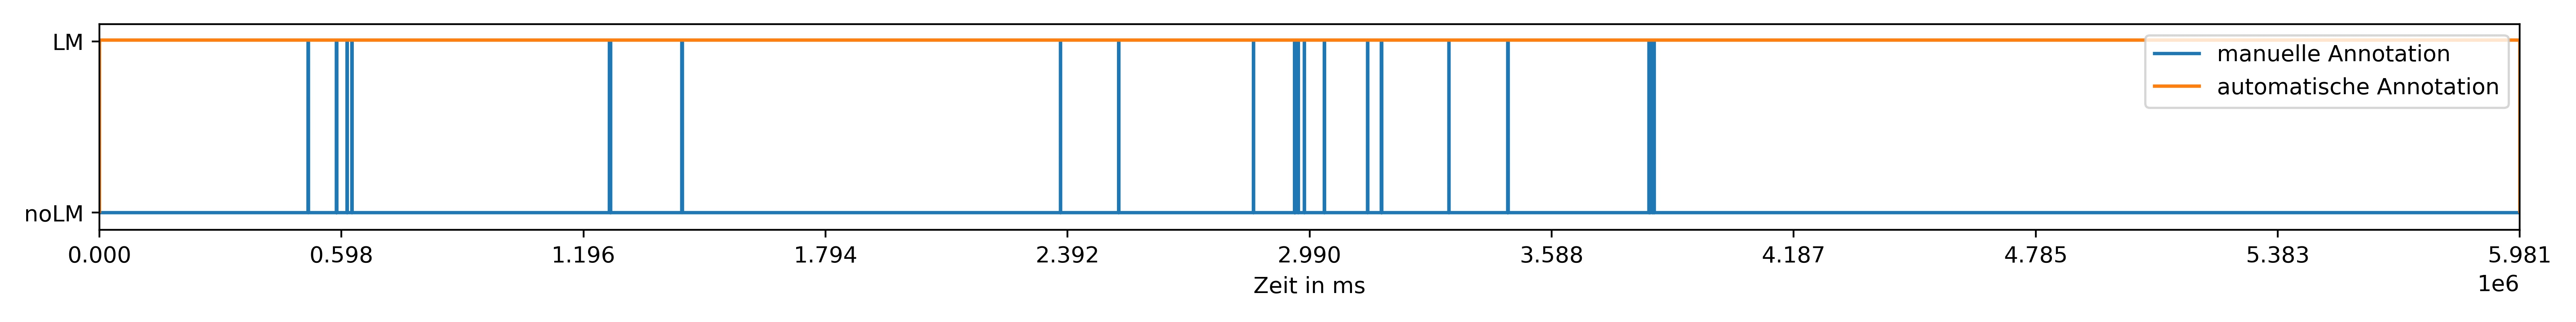
\includegraphics[width=0.80\textwidth]{./Bilder/customAll1.jpg}
	\end{center}
	\caption{Beispielannotation bei der die automatische Annotation nur positiv ist. Es entstehen Kosten von vier obwohl klassische Metriken Eins sind.}%
	\label{fig:all1}%
\end{figure}


In dem Beispiel \ref{fig:all0} wurde die automatische Annotation auf null gesetzt für die gesamte Nacht. Das Kostenfunktional kommt hier wieder auf einen Wert von 4 und auf relative Kosten von Eins. Die Genauigkeit und falsch positiv Rate sind in diesem Fall nicht definiert, da Zähler und Nenner Null sind. In diesem Fall werden die Metriken teilweise auch als Eins also als perfekte Genauigkeit definiert \cite{glassbox}. Laut Spezifität ist ein Detektor, der trivialerweise immer Null ausgibt also auch perfekt. 

\begin{figure}[!ht]%
	\begin{center}
	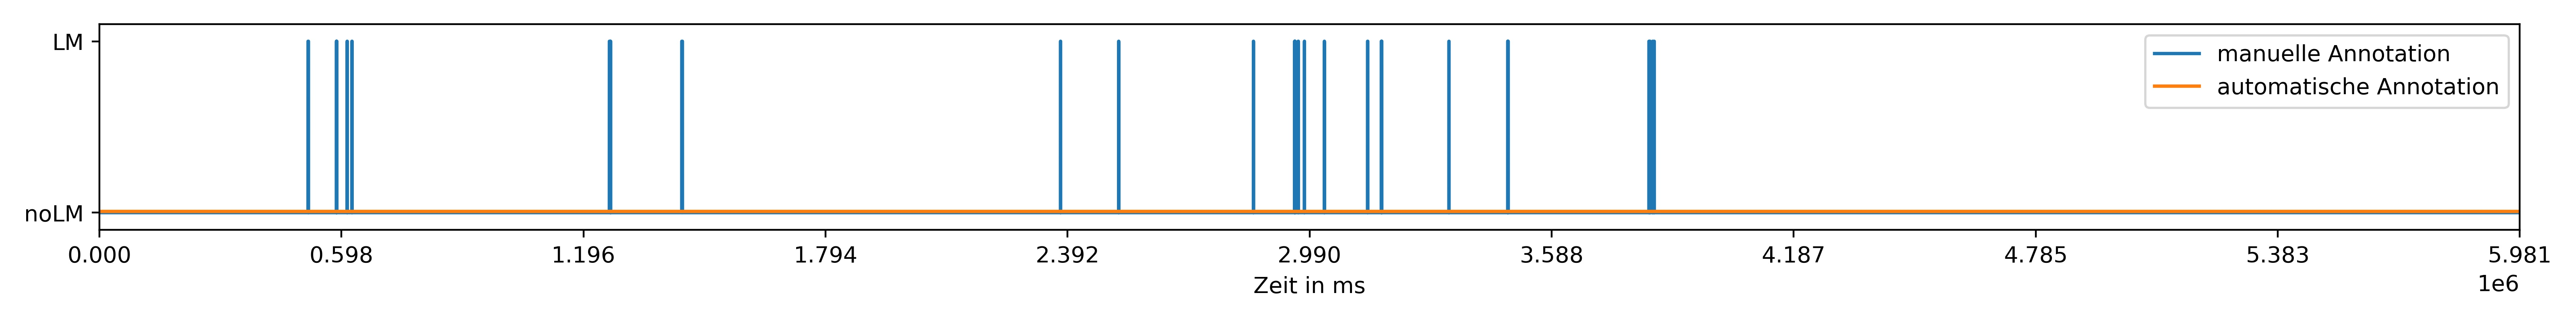
\includegraphics[width=0.80\textwidth]{./Bilder/AllZero.jpg}
	\end{center}
	\caption{Beispielannotation bei der die automatische Annotation nur negativ ist. Es entstehen Kosten von vier obwohl klassische Metriken Eins sind.}%
	\label{fig:all0}%
\end{figure}

Für einen Detektor, der die manuelle Annotation exakt nachbildet, wie in Bild \ref{fig:same} dargestellt, wären beide Annotationssignale identisch. Da hier keine Fehler gemacht werden sind die absoluten und relativen Kosten Null. Die Güte hat somit den perfekten Wert von Eins.

\begin{figure}[!ht]%
	\begin{center}
	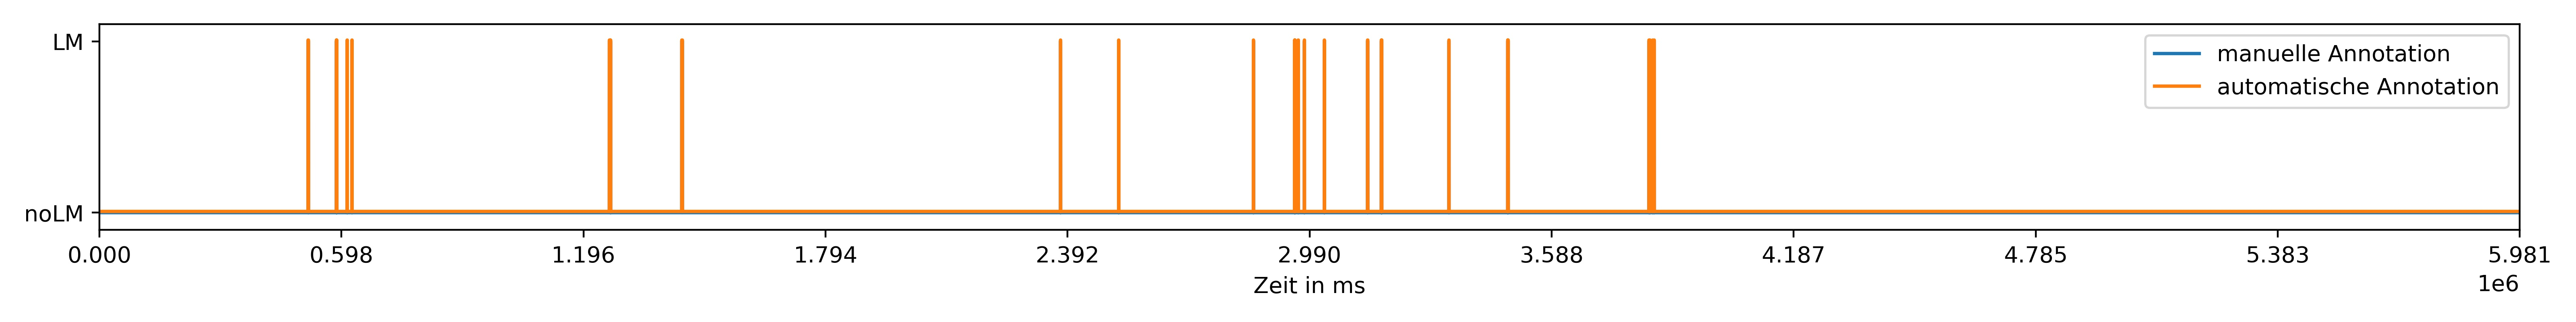
\includegraphics[width=0.80\textwidth]{./Bilder/aAnno=mAnno.jpg}
	\end{center}
	\caption{Beispielannotation bei der die automatische Annotation identisch zur manuellen Annotation ist. Die Güte des Detektors wäre in diesem Beispiel Eins.}%
	\label{fig:same}%
\end{figure}

Für die nachfolgenden Ergebnisse wurden Annotationssignale selbst erstellt, damit die einzelnen Kostenbeiträge besser veranschaulicht werden können.
Die Funktionsweise der multiplen Zuordnung lässt sich in Abbildung \ref{fig:Xto1} veranschaulichen. In dem Beispiel wurden der einen automatischen Annotation vier manuelle zugeordnet. Die absoluten Kosten sind wieder vier, da keins der vier manuell gefundenen PLM entdeckt wurde. Alle klassischen Metriken würden anhand dieses Signals einen perfekten Wert ausgeben. Das 1toX-Matching lässt sich analog darstellen. 

 
 \begin{figure}[!ht]%
	\begin{center}
	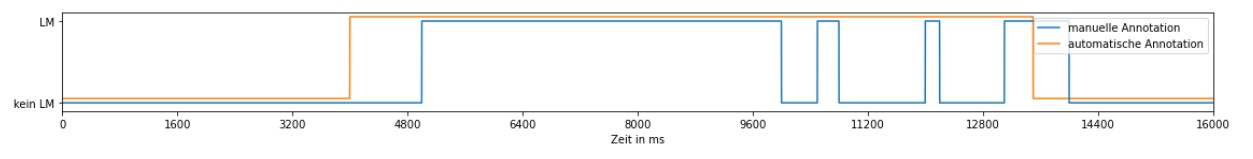
\includegraphics[width=0.80\textwidth]{./Bilder/Xto1.jpg}
	\end{center}
	\caption{Beispielannotation bei der die automatische Annotation einen Fehler durch Xto1-Matching aufweist.}%
	\label{fig:Xto1}%
\end{figure}

In Abbildung \ref{fig:FP} wird der Fehler aufgrund eines \gls{FP} dargestellt, welcher somit eine Serie feststellt, obwohl die manuelle Annotation keine PLM erkennt. Die Kosten sind hier ebenfalls vier.
\begin{figure}[!ht]%
	\begin{center}
	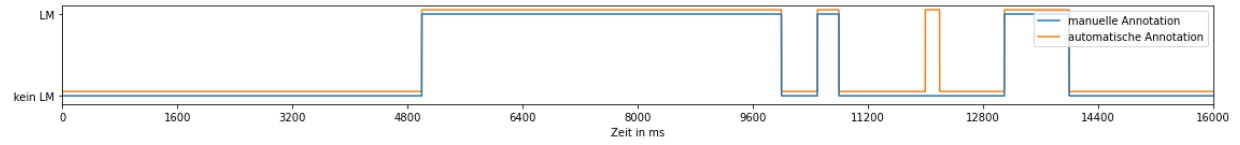
\includegraphics[width=0.80\textwidth]{./Bilder/FP.jpg}
	\end{center}
	\caption{Beispielannotation bei der die automatische Annotation einen Fehler aufgrund eines \gls{FP} aufweist.}%
	\label{fig:FP}%
\end{figure}

Die Abbildung \ref{fig:timevio} zeigt, dass eine zeitlich ungenaue Annotation in dem letzten LM ebenfalls zu einem Fehler führen kann. Hier erfüllt das LM der manuellen Annotation nicht die von der AASM geforderten Zeitbedingungen um als PLM zu zählen. 

\begin{figure}[!ht]%
	\begin{center}
	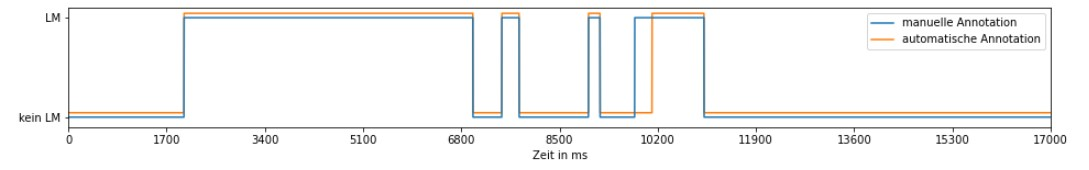
\includegraphics[width=0.80\textwidth]{./Bilder/TimeVio.jpg}
	\end{center}
	\caption{Beispielannotation bei der die automatische Annotation einen Fehler aufgrund eines ungenauen Startwertes aufweist.}%
	\label{fig:timevio}%
\end{figure}

In dem Beispiel \ref{fig:0.2Kost} wurde das letzte LM nicht erkannt und der Fehler aufgrund \gls{FN} beträgt Eins. Die relativen Kosten sind hier nur 0.2, da trotzdem vier der fünf LM in der PLM-Serie richtig erkannt wurden.


\begin{figure}[!ht]%
	\begin{center}
	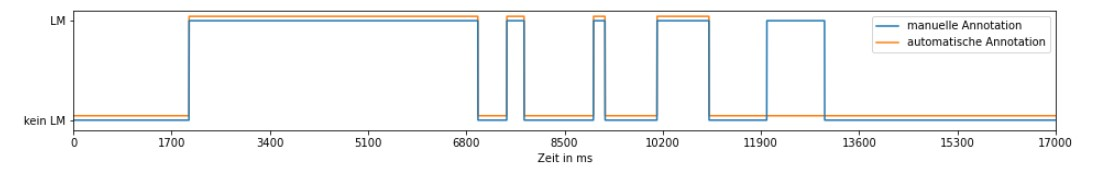
\includegraphics[width=0.80\textwidth]{./Bilder/0.2Kost.jpg}
	\end{center}
	\caption{Beispielannotation bei der die automatische Annotation einen Fehler aufgrund eines FN aufweist. Es entstehen relative Kosten von 0.2.}%
	\label{fig:0.2Kost}%
\end{figure}

Im Bild \ref{fig:achtKost} ist dargestellt, wie bei dem ersten automatisch erkannten LM ein Xto1-Matching vorliegt. Dieses wird aber gleichzeitig in eine weitere PLM-Serie aus FP gezählt. Obwohl die PLM Anzahl für beide Annotationen gleich ist, entstehen hier absolute Kosten von acht und relative Kosten von zwei. 

\begin{figure}[!ht]%
	\begin{center}
	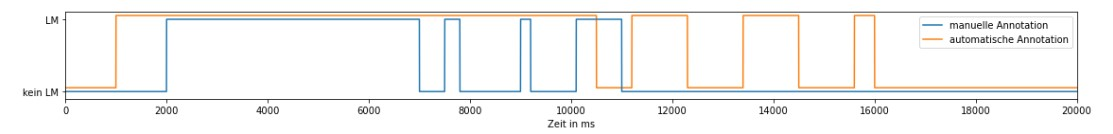
\includegraphics[width=0.80\textwidth]{./Bilder/underovercount.jpg}
	\end{center}
	\caption{Beispielannotation bei denen Kosten entstehen, obwohl die PLM Anzahl gleich ist. Es entstehen absolute Kosten von Acht.}%
	\label{fig:achtKost}%
\end{figure}




Falls es keine anderen außer die oben genannten Fehler gibt, müsste
\begin{equation}
\overset{\text{ergebniserhöhende Fehler \textminus \ ergebnisverkleinernde Fehler}}{\underset{\text{automatisch annotierte PLM \textminus \ manuell annotierte PLM}}{=}}
\label{kdiff}\end{equation}
gelten. Diese Gleichung beschreibt alle Fehler, die durch das Kostenfunktional gefunden werden können und setzt diese in Beziehung zu den tatsächlich auftretenden Fehlern. Mit dieser Gleichung kann also überprüft werden, ob alle einzeln gemachten Fehler auch gefunden wurden.

Es gibt jedoch auch Detektorfehler, die das Ergebnis nicht verändern aber trotzdem als Kosten zählen sollen. Zum Beispiel kann es passieren, dass eine manuell gefundene PLM Serie durch einen Zeitfehler (siehe Punkt 2) in zwar aus der einen Serie exkludiert wird, aber in einer anderen Serie damit inkludiert wird. 
Da sowohl Verkleinerung als auch Vergrößerung des Ergebnisses als falsch zu beurteilen ist, werden beide Fehlerarten addiert und bilden damit das Kostenfunktional: 
\begin{equation}
K_{abs} = ergebniserhöhende\ Fehler + ergebnisverkleinernde\  Fehler     
\end{equation}

Die absolute Anzahl an Fehlern kann bei unterschiedlichen Datensätzen irreführend sein, da zwar die Wahrscheinlichkeit einen Fehler zu machen gleich sein sollte, aber bei mehr Events auch mehr Fehler entstehen. Daher sollte das Kostenfunktional auf die Anzahl der manuell annotierten PLM in der jeweiligen Serie normiert werden. Somit sind die Kosten auch unabhängig von der durchschnittlichen Länge der PLM-Serien. Das finale Kostenfunktional stellt also dar wie viele Fehler pro richtig erkannte PLM gemacht werden.


\section{Verbesserung der Einordnung des Detektors}\label{Verbesserung}


Dieses Kapitel bezieht sich darauf weitere nützliche Information aus den Annotationssignalen zu extrahieren, um mit diesen den Detektor besser einschätzen zu können. Diese Metriken gehen nicht in die Berechnung der Güte ein, können aber informativ genutzt werden.

Da sich die anderen Metriken hauptsächlich auf einzelne LM beziehen, könnte eine Metrik nützlich sein, welche große Veränderungen der Annotationen im Laufe der Nacht, darstellt. Diese könnte durch den Schwerpunkt der Startzeitpunkte der LM berechnet werden. Da das Gewicht jedes LM eins ist, und der Abstand gleich des Startzeitpunktes ist, geht die Berechnung des Schwerpunktes in die des Mittelwertes über.
Dieser Wert könnte dafür genutzt werden, große Veränderungen, bei denen sich die Annotation im Laufe der Nacht ändert, zu erkennen. Interessant ist auch, ob diese Veränderung von beiden Annotationen gleichermaßen detektiert wurde. Also berechnet sich die Metrik aus der Differenz der beiden Schwerpunkte.

Eine weitere Information steck in der zeitlichen Genauigkeit der Start- und Endzeitpunkte der Beinbewegungen. Diese lassen sich nur bei der eventweisen Zuordnung von Beinbewegungen zu TP analysieren. 
Falls eines der beiden Annotationssignale segmentweise ausgewertet wurde, geht genauere Information zu den Startzeitpunkten verloren. Diese Genauigkeit könnte in dem anderen Annotationssignal höher sein. Betrachtet man nun die Differenz der jeweiligen Startzeitpunkte von TP entsteht eine Verteilung. Die nächsten beiden Metriken beschreiben also den Mittelwert und die Standardabweichung dieser Verteilung. Da die Wahrscheinlichkeit des zeitlich höher aufgelösten Annotationssignal ein LM-Start zu haben unabhängig von den Segmentgrenzen des andren Annotationssignals ist, liegt der Erwartungswert bei null.
Analog lässt sich auch eine Verteilung für die Endzeitpunkte der LM berechnen.

Eine hohe Anzahl an FP in einzelnen Nächten könnte darauf hindeuten, dass Events manuell entweder nicht betrachtet wurden oder nach einer Annotation im Nachhinein wieder gelöscht wurden. Die klassische Metrik der falsch positiv Rate könnte ein Indiz über diese Art von Uneinigkeit geben.

Des Weiteren lassen sich Information gewinnen, welche genutzt werden kann, um die Arbeitsweise des Detektors besser zu verstehen, um den Detektor gegebenenfalls zu optimieren.
So kann beispielsweise das Verhältnis aus der Anzahl automatisch gefundener LM zu der Anzahl manuell gefundener LM darauf hindeuten wie schnell der Detektor auf positive Änderungen im EMG reagiert. 


Eine Verwandte Information liefert die Anzahl der multiplen Zuordnung (Xto1- und 1toX-Matching). Diese Werte könnten beschreiben wie schnell der Detektor auf eine negative Änderung im EMG reagiert. 

Da Beinbewegungen laut AASM eine bestimmte Mindest- und Maximaldauer haben, könnte die Zahl der Verstöße gegen diese Zeiten aufschlussreich über die Art der gefundenen Muskelkontraktionen. 

Diese Informationen sind allerdings nur im Kontext der Funktionsweise des Detektors nützlich und sollten nicht zur Bewertung verwendet werden.

In der Grafik \ref{fig:Metriken} sind die nützlichen Informationen zum Detektor dargestellt. Der obere Kreis bezieht sich auf den Vergleich zu bisherigen Detektoren. Hierfür sind die angegebenen klassischen Metriken am nützlichsten, da diese von den bisher entwickelten Detektoren angegeben wurden. Diese können außerdem einen guten Überblick darüber geben, wie viele von den Beinbewegungen circa richtig erkannt werden. Besonders Cohens $\kappa$ und das F1-Maß treffen eine vergleichsweise genaue Aussage.
Links im Bild sind die Informationen zu dem Detektor dargestellt, welche Aussagen über die Funktionsweise des Detektors liefern.
Der rechte Unterpunkt beschreibt das Kostenfunktional und seine Einflussfaktoren.
\begin{figure}[!ht]%
	\begin{center}
	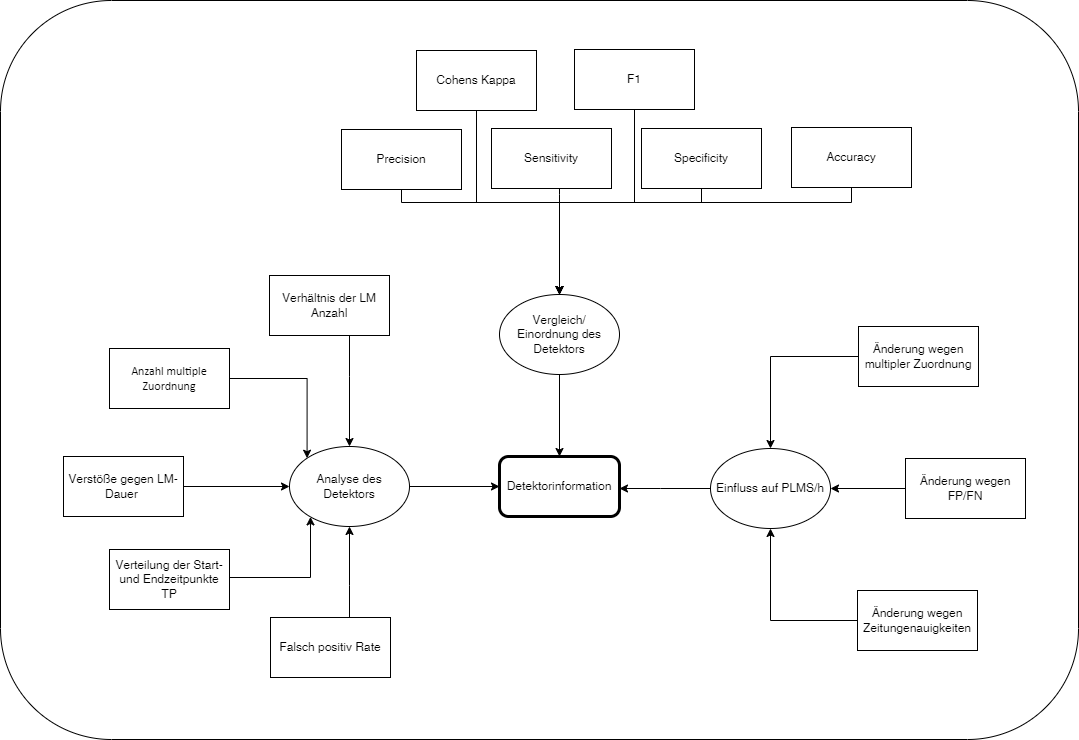
\includegraphics[width=0.80\textwidth]{./Bilder/Metrik.png}
	\end{center}
	\caption{Darstellung der Metriken, die zum Informationsgewinn oder zur Bewertung des Detektors verwendet werden können.}%
	\label{fig:Metriken}%
\end{figure}